\documentclass[10pt,letter,oneside]{scrartcl} 
\usepackage{setspace}
\usepackage[utf8]{inputenc} 
\usepackage[english]{babel}
%\usepackage{raleway} \renewcommand*\familydefault{\sfdefault} %% Only if the
%base font of the document is to be sans serif
\usepackage{graphicx} % Required for including images 
\usepackage{enumitem} 
%Required for manipulating the whitespace between and within lists
\usepackage[T1]{fontenc} % Use 8-bit encoding that has 256 glyphs
%\usepackage{natbib}
\usepackage{breakurl} 
\usepackage[breaklinks]{hyperref} 
\usepackage{pdfpages}
\usepackage{endnotes} \let\footnote=\endnote

\usepackage[style=authoryear]{biblatex} 
\addbibresource{hack_entry.bib}

\usepackage{authblk} 
\author[1]{Luis Felipe Rosado Murillo}
\author[2]{Christopher Kelty} 
\affil[1]{Berkman Center for Internet and Society, Harvard University} 
\affil[2]{Institute for Society and Genetics,
          Department of Anthropology, and Department of Information Studies, UCLA}
\renewcommand\Affilfont{\itshape\small}

\title{Hackers and Hacking}

\date{}

\begin{document} 
\maketitle 
% \section*{Abstract} 

\doublespacing 

\section*{Introduction}

Hackers seem to be everywhere today.

\begin{figure}
  \centering
  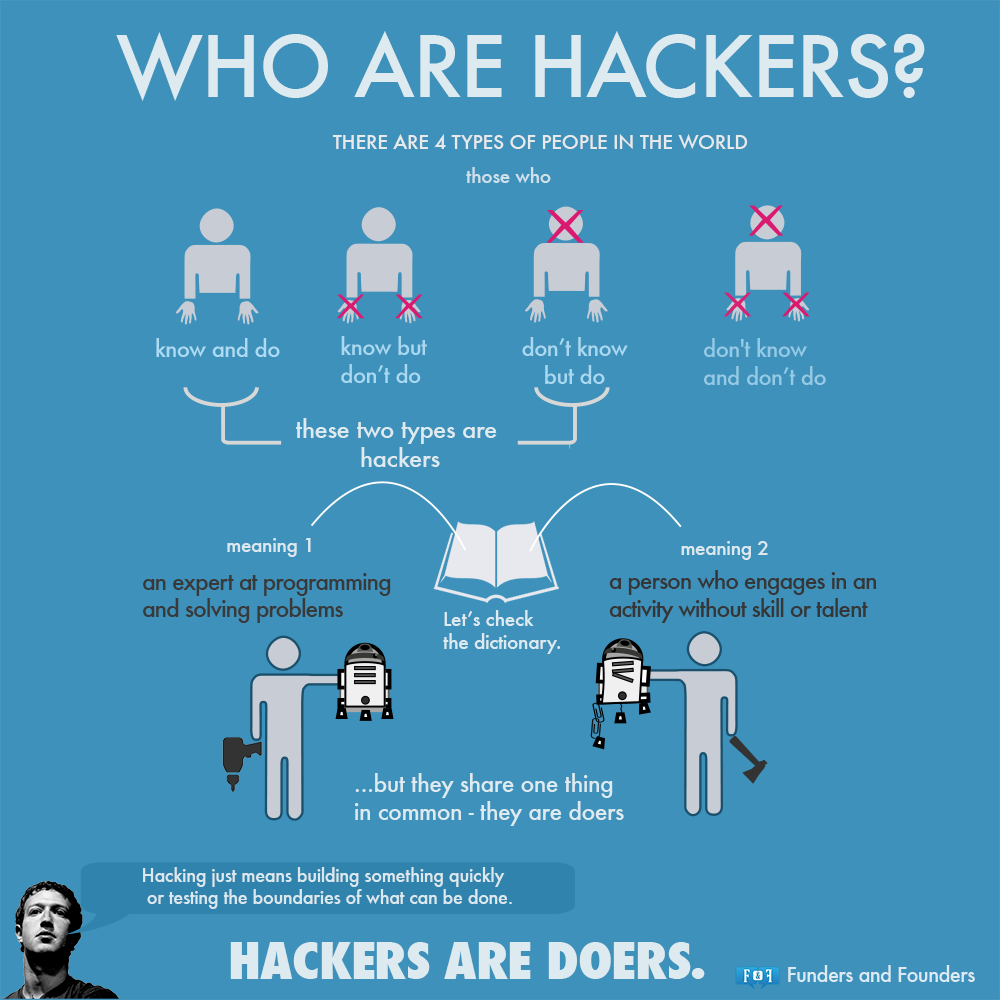
\includegraphics[scale=0.3]{images/Hacker-doers}
  \caption{"Hackers are Doers" Funders and Founders Website \parencite{funders_2016}}
  \label{fig:doers}
\end{figure}

Twenty five years ago, ``hacking'' was one of a range of underground practices,
associated with a particular politics and defining a set of individuals usually
characterized as adolescent, white males obsessed with computers.  Today,
literally anyone could call themselves a hacker, or any action a ``hack.'' In
recent decades, we have experienced the extension of the term to encompass many
ordinary technical practices in various domains, such as education, health care,
humanitarian response, farming, parenting, bodily modification, among many
others.  In Silicon Valley, companies like Facebook describe a ``hacker way'' to
reference ordinary practices of coding, engineering, or entrepreneurship.  In
public relation campaigns, hackers are described simply as ``doers'' since
``hacking just means building something quickly or testing the boundaries of
what can be done'' (See fig \ref{fig:doers}. According to this very generous
definition, we can all be called ``hackers'', since we have been making
artifacts for, at least, 2 millions years with the creation of mode-1 stone
tools \parencite{clark_world_1961}.

We have also witnessed a proliferation and globalization of hackfests,
hackathons, hackerspaces and gatherings around the symbol of hacking for a
myriad of purposes, including but not limited to the design of open hardware
devices in medical settings, the corporate-sponsored challenge of reinventing
the soda fountain with support from big companies such as Coca-Cola, the
collective work around public data-sets to fight corruption or help with
questions of public administration, or simply coming up with an inventive use of
a product that is about to be released in the market.  Hacker conventions---like
conferences in academic settings---serve the purposes of exchanging knowledge
and bringing small and fringe groups of computer aficionados together to find
peers, to share questions and findings that emerge when playing and working with
information and communication systems \parencite{coleman_conference_2010}.  In
the contemporary, many ``hacker marathons'' have been organized by companies to
identify programmers for hire, offering comparatively small sums as prizes for
new software or hardware solutions which would necessarily cost considerably
much more in research and development.  A new business has been created around
the work of head-hunting for software engineering talent under the rubric of the
``hackathon,'' despite its original connotation of a community-led sprint for
developing technologies.

These facts suggest that the figure of hacking and hackers has become
fundamental to a contemporary technopolitical imaginary.  Whatever hacking is,
it is a very appealing figure and explanation for something.  Hacking has become
both a rubric for something very general, while at the same time designating a
very specific set of practices from specific genealogies.  In this article we
explore some of the ways hackers and hacking have been studied by academics, as
well as the forms of self-narration that different hacker groups have themselves
forged.  We argue that the subjectivities involved in cultivating ``hacking
skills'' are not implicated in the range of things that can be called
``hacks''---or put differently: these days not all hacks are perpetrated by
hackers.  We then ask what the relationship is between \emph{hackers} as a
particular elaboration on what it means to be a person, and \emph{hacking} as a
particular practice.  We end by suggesting one possible way to decompose hacking
into a ``stack'' of practices that can be used to diagnose technical and
political thresholds indicative of a mutation in the ``topology'' of power in
the world today.  Or to put it differently, there is a reason why hacking seems
to be spreading everywhere: because the forms and affordances of technical and
political power are themselves changing, and hackers are at one forefront of
experimenting with such mutations.

\section*{Stories of Hackers and Hacking}

From the early 1950's experimentation with communication and computing systems
to the present-day hacker activist initiatives in the Global North and South,
the narratives of hacking have been given different genealogies, supporting
different positionings with respect to who and what counts as a legitimate
expression of hacking.  Most of these influential narratives have been provided
by journalists and self-designated hackers, but canonical scholarly works
generally focus on the ``culture'' of computing---and not specifically about
hacking: Sherry Turkle \cite*{turkle_life_1995,turkle_second_1984}, Diana
Forsythe \cite*{forsythe_studying_2001}; David Hakken and Barbara Andrews
\cite*{hakken_computing_1993}; Lucy Suchman \cite*{suchman_plans_1987}; Star and
Ruhleder \cite*{star_infrastructure_1996}; Stephen Helmreich
\cite*{helmreich_silicon_1998}; Joseph Dumit \cite*{dumit_picturing_2004}, and
Greg Downey \cite*{downey_machine_1998}. At the most basic level, this
literature has helped to address the so-called ``myth of autonomous technology''
which presupposes a modernist ontology which separates it from human culture and
society \parencite{latour_wehave_2008,winner_auto_1978,}.  Pfaffenberger
\cite*{pfaffenberger_social_1992} pioneered the anthropological study of
sociotechnical systems in this tradition by refusing a separation between
technology and culture. In his studies of digital technology (such as the Usenet
and the Personal Computer), he argued for the processual analysis of
technological design as invariably embedded in cultural systems. With the
exception of Pfaffenberger and Turkle, little of this scholarly work is directly
focused on hackers or hacking as such, but nonetheless constitutes some of the
most significant ethnographic studies of computing in English-language.


The journalist Steven Levy is one of the most authoritative sources on the early
history. His mid-1980's book \emph{Hackers: Heroes of the Computer
  Revolution} \parencite{levy_hackers:_1984} is exemplary in offering early
heroic narratives of the exploration of computer systems. It is based on
life-histories, tracing the origins of the hackerdom to the ``Tech Model
Railroad Club'' (TMRC) of the Massachusetts Institute of Technology (MIT) of the
1950's. \emph{Hackers} has been translated into several languages and accepted
among distinct hacker communities worldwide.  Its narrative had the performative
force of instituting a return to the figure of the ``virtuous hacker''through
descriptions of the experience of early hackers at MIT and Stanford, in Northern
California collectives such as ``People's Computer Company'' and ``Homebrew
Computer Club'', and companies such as Apple Computer and Sierra Games.  Levy
has also popularized a positive definition of hacking as grounded in the
``hands-on imperative'' and the ``hacker ethic.''  This ethic includes the
commitment to information freedom to facilitate technical exchange and to
promote further hacking; a rebellious attitude with respect to authority,
centralization, and control of computing infrastructures; and the idea that
technical work could be used to bring forth beauty and effect positive social
change.  Similar stories are told in the widely read books \emph{Where Wizards
  Stay up Late} \parencite{hafner1998wizards} and later in \emph{Hacker Ethic
  and the Spirit of Information Age} by the Finnish philosopher Pekka Himanen
(2001). While the former offered a heroic tale of the early days of the Internet
engineering research, the latter was calling attention to the subjective
dimensions of a cultivation that is distinctive of the computer hacker ascesis.

A more recent account of the early origins of hacking was given by the
technologist Phil Lapsley \cite*{lapsley_exploding_2013} in his book
\emph{Exploding the Phone: The Untold Story of the Teenagers and Outlaws who
  Hacked Ma Bell} which reconstructed the early history of ``phone-phreaking'',
the precursor of computer hacking which consisted in the exploration and
information sharing about phone systems.  Lapsley describes a genealogy which
connects the direct action of Yippies of the 1960's with exploration of
information and communication systems in the context of corporate control and
centralization of computing in the 1960's and 1970's.  His account calls
attention to a fundamental aspect of phone phreaking: a shared experience in
which the telephone became the very embodiment of curiosity, and the phone
network, a space for exploration, discovery, and socialization.

% This is an important period of transition of the past 50 years in which we have
% witnessed the passage from large-scale, military-grade computer infrastructures
% to distributed personal computing power with massive network integration in the
% Euro-American world. The consequences of this transition are key for the study
% of digitization: the transformation of cultural practices through the usage of
% digital technologies, difference in infrastructure (of computing networks),
% materiality (of computing devices), and virtuality (of archival and social
% memories).

A distinctive feature of hacker collectives resides in their effort of
self-organization around publications and gatherings.  Akin to other independent
groups, many phone-phreaking and hacker groups engaged in the practice of
self-documentation, with the publication of ``electronic zines'', manifestos,
and, in a few cases, with the enthusiastic adoption of an anthropological and
historiographic mode of inquiry.  Jason Scott (see Appendix) has emerged as a
self-appointed archivist of much of this material, maintaining extensive
archives of natively produced electronic documents, series of life-histories on
hacking, Bulletin Board Systems (BBS), and adventure, text-based games and much
else.  Eric Raymond, a well-known hacker and writer is also regarded by many as
a native anthropologist of hackerdom, having written on the culture and language
of hackers, and the moral norms associated with open source and free software
\parencite{raymond_cathedral_1999,raymond_art_2004}.  Raymond did much to preserve
and popularize the collaboratively produced document known as the ``Jargon
File'' which documented the rich language of early internet, usenet and hacking
terminology, and was republished as \emph{New Hackers Dictionary}
\parencite{raymond_new_1993} (see further reading).

Two major sociological and historiographic contributions in the literature
depicting the rise and fall of the "hacker underground'' of the 1980's and
1990's were ``Hacker Culture'' by the communications scholar Douglas Thomas
\cite*{thomas_hacker_2002} and ``Hackers'' by the sociologist Paul Taylor
\cite*{taylor1999hackers}. These two books are complementary in the sense that
they describe the underground hacker scene of the United States and the United
Kingdom in the period of popularization of hacker techniques and criminalization
of its practice.  Taylor's work is focused on the relationship between the
nascent computer security industry of the 1990's and the computer underground,
giving a fruitful description of the duality which is characteristic of the
underground lifeworld in which hackers are ambiguously the chaser and the chase,
both on the side of law enforcement and on the side of the curious hacker
collectives.  Douglas' work is particularly useful in describing the discursive
strategies in which the figure of the hacker as a unpredictable and
uncontrollable ``criminal'' was instituted -- having created a mythology around
the alleged superpowers of curious adolescents with access to a personal
computer, a modem, a phone line and certain access to information about flaws
and holes in computer and communication security.

The work of the science-fiction writer Bruce Sterling alongside others in
creating the ``cyberpunk'' literary genre led him to cross paths with hacker
groups in the United States in a key moment of its history: the late 80's and
early 90's in which the wave of ``crackdown'' on hacker collectives has become
widespread, especially in the wake of the US Computer Fraud and Abuse Act (CFAA)
of 1986. His book ``Hacker Crackdown'' narrates the story of police chase after
teenage hackers \parencite{sterling_crackdown_1993}.  Key in his depiction is
the argument of how misguided the police attempts were in framing computer
hacking as a serious criminal offense without understanding of the practice and
its consequences.  This period also saw the rise of several media darlings and
misfits, the most famous being Kevin Mitnick, who became the mainstream media
martyr after an incredible story of playing cat-and-mouse with the federal
police in the United States.  After being arrested, a mobilization of hackers
around the slogan ``Free Kevin'' took over the computer underground to clarify
the misguidance and overreach of prosecutors in Mitnick's case.  Many other
hackers' stories rose to prominence in this period, including the hacker
collective Legion of Doom (LOD) and their New York-based rival offshoot Masters
of Deception (MOD).

In the 2000s, scholarly attention to hackers and related communities of computer
users picked up significantly, especially around Free and Open Source Software
on the one hand and online gaming on the other (the latter being too large a
field to touch on here, but see \textcite{coleman_review_2010a}).  Hackers in
free software projects formed the subject of work by Kelty, Coleman, Karanovic,
Hakken and
others\parencite{kelty_two_2008,coleman_coding_2012,auray_debian_2003,broca_utopie_2013}.
This literature connected work on hackers directly to issues of intellectual
property and activism around it on the one hand, and also to questions about the
liberal underpinnings of Free Software and the question of the putative
liberalism and/or libertarianism of hackers themselves in the Euro-American
context.  Golub and Coleman \cite*{coleman_hacker_2008} argued most explicitly
for refining our understanding of the differences \emph{within} hackerdom by
proposing several ``genres'' of hacking to get at distinctions with respect to
the moral and technical orders different hacker groups inhabit.

More recent publication and public debates around Free Software and hacker
communities has shifted the focus to questions of gender discrimination and
imbalance.  Alongside the work of feminist and women hackers around computer
collectives such as Systers, LinuxChix, Ada Initiative and Geek Feminism, new
publications have addressed the question of extreme disparity in Free and Open
Source projects where it is estimated that less than 2\% of the contribors are
women and other gender minories \parencite{ghosh_understanding_2005}.  Nafus
\cite*{nafus_patches_2012} has discussed the question of gender with respect to
the ways in which the organizing symbol of ``openness'' represents more than an
alternative to the intellectual property regime and a mode of managing the
collaborative efforts in software development.  According to the author, the
question of openness is accompanied with the insistence that gender plays no
role in software development, serving in fact to disguise the mechanisms of
exclusion of women and gender minorities from Free and Open Source projects.

% These mechanisms include but are not limited, to the maintenance of design
% decisions which demand previous technical knowledge, excluding newcomers; the
% creation of new expressions of masculinity that are exercised through public
% argumentation and defense of one's technical prowess, which are alienating to
% women and other gender minorities; and, last but not least, one of practical
% effects of ``openness'' which consists in denegating or outright denying
% ``difference'' for the sake of unfettered circulation of code, which has the
% effect of generating ``flame-fests'' when the question of gender is posed for
% debate among FOSS developers.

The most recent publication on the topic of ``hacking'' includes work by Michel
Lallemand on the topic of ``hackerspaces'' and the rise of the discourse and
practice of ``making'' \parencite{lallement}.  Lallemant has offered an ethnography
of the ``maker movement'' in the San Francisco Bay Area with a focus on the
question of the transformations labor and its reorganization with the creation
of independent spaces for collaborative work with digital technologies. The book
describes the community space ``Noisebridge'' in San Francisco which has been
one of the most influential autonomous spaces for the recreation of hacking as a
political symbol for self-organization and wider access to expert computing 
knowledge around the globe.

\section*{Hackers...}

One of the key insights of recent anthropology of hackers in the Euro-American
context is how they represent a distinctive elaboration of
liberalism---especially in the domains of free speech and the cultivation of a
self directed towards freedom, autonomy, privacy and other liberal
values \parencite{coleman_coding_2012,kelty_two_2008,coleman_hacker_2014}. Hackers
are not uniformly libertarian or simply privacy advocates, but articulate a
relationship to technology with a different range of values depending on their
``genre'' \parencite{coleman_hacker_2008}. Little work has been done on the way
this relation to technology articulates with different political and
philosophical traditions outside the Euro-American world, though a handful of
people have advanced such questioning
\cite{xiang_2007,takhteyev_coding_2012,chan_networking_2013}.

Complicating this question of the productive relation to technology, however, is
the question of whether ``hacking'' is a specific practice, skill or domain of
knowledge.  How are hacks valued and assessed, and how they are shared, learned,
improvised, recorded and displayed, or circulated?  Hackers are said to have a
culture of perpetrating a particular kind of act which can supposedly be
distinguished from the actions of other kinds of people in other professional
domains (especially, those in bureaucracies, corporations, or other hidebound
organizations of the past).  The ``hack'' however, can be mobile and re-usable,
it often, but not always, takes the form of a tool or set of tools; it can be a
one-off, round-about way of getting something done, but it is often something
that is re-usable, which serves as yet another element for generalization.  Many
ordinary practices of repurposing, in different contexts, have different
expressions, such as the ``gambiarra'', the Brazilian term for an improvisation
of and deviation technical knowledge, the ``juugad'', which expresses a similar
improvisation of technical nature in India, and the ``shanzhai'', which is a
more specific form of repurposing mobile devices in mainland China.

% maybe also the Amish...  

In these cases, the ``hacker'' persona is troubled by the recognition that
``hacks'' are frequently borrowed, re-used, reconfigured and redeployed by
people who only subsequently come to self-identify as hackers---or maybe
don’t do so at all.  Conversely, depending on the context of occurrence and the
participants of the exchange, you could be called a hacker regardless of your
expertise, but solely on the basis of the technical feat you have performed.
Hacks are contextually visible to hackers, and depend on such assessment and
attribution to legitimately be called hacks.

The tension in hacker personhood arises when someone claims to be a hacker,
but of an unfamiliar sort.  Most classic hackers hew to a definition of hacker
that is open to inclusion in a particular way: through the convivial but
competitive demonstration of skill in hacking.  The definition of what can be
included as a hack is always extensible, but only by demonstration to some set
of witnesses capable of judging it.   So when the word "hack is used to refer
to something that does not seem to manifest particular skill or convivial
competitiveness, then a tension emerges. 

Such a complicated identification of who counts as a hacker poses a dual problem
for anthropological research.  On the one hand, it creates a challenge for
making sense of personhood itself in a domain where conventional idioms of what
it means to be a hacker are highly contested and subjected to critique and
extension.  In particular, hackers are often fond of rejecting the traditional
credentials of schools, employers, states or other entities that confer
expertise; they prefer the recognition of the hack itself. On the other hand,
our anthropological attention can be directed to the act
itself---``hacking''---and to the question of what it is and how it might be
studied anthropologically, or for instance, with the tools of science
studies. When are the actions of pirates, activists, criminals, spies and other
such figures considered ``hacks''?  When do people call mid-level engineers,
librarians, scholars and designers ``hackers'' and when not?  Do all of these
people, with a wide range of computing expertise, share a particular set of
cultivated dispositions, or do they share a milieu of technical devices and
communication infrastructures at their disposal?  How can we disentangle the
sudden dispersal of hacking and hackers, in the sense of a wide circulation of
devices, persons, and discourses, around the world?

As we briefly explored in the previous section, there have long been competing
definitions of hackers.  Consider two distinctive definitions: one from the
Internet engineering community and the other from ``hacker underground.''  For
the former, a hacker is defined as a person ``who delights in having an intimate
understanding of a technological system,'' whereas his or her opposite, a
``cracker,'' is an individual who attempts to access computer systems without
authorization.  These hackers pride themselves on building complex systems out
of available parts, or on getting around an engineering problem in a simple and
elegant way--and they deride ``crackers'' as adolescents with only enough
knowledge to cause trouble.  As Coleman \cite*{coleman_coding_2012} details,
they are highly individualistic (in the Euro-American context), but strongly
oriented towards a community of other hackers---as in the case of Free Software
hackers. 

By contrast, for underground hacker collectives, hacking may signify exclusively
``systems' penetration'' and exploitation of vulnerabilities as a display of
technical ability and mastery or, increasingly, for monetary gain.  For them,
hackers are people ``who gain unauthorized access to computer systems,'' a
practice which is evaluated in terms of technical aptitude and virtue, measured
up against the value of contributions in software code, information, and
documentation.  ``Exploits'' become objects of value that circulate---at one
time only for a kind of cultural capital amongst hackers, but increasingly today
as part of a robust market for ``zero-day'' exploits.  Increasingly, these forms
of hacking are also well established in the military and defense world, both
defensively and offensively in geopolitical arenas.

Members of the early Internet engineering expert communities claiming the hacker
status would strongly disagree with the definition given by or of the hacker
underground. Many of these communities were described in the origin stories of
Free and Open Source development as a ``natural attitude'' of pioneer computer
technologists.  They are strongly associated with research universities and with
a Mertonian understanding of scientific practice; they point back to avatars
such as the Digital Equipment Computer Users' Society (DECUS) in the sixties, or
SHARE, the IBM mainframe computer users' group \parencite{akera2001voluntarism},
the MIT community around the Tech Model Railroad Club, the Artificial
Intelligence Laboratory operating system development staff, and the early
community around Berkeley Unix System distribution (BSD), among many others.
The period which extends from the 1950's to the 1970's is identified in the
literature with the work of early, pioneer hackers in pushing the boundaries of
computing on many fronts: from hardware hacking to personal computers, from new
operating systems to video-games and graphical user interfaces as we discussed
above.

By contrast the ``hacker underground'' has its own mythical histories,
associated with the history of phone phreaking, bulletin board systems (BBS),
zines like ``2600'' and ``Phrack'', and movies like \emph{War Games} and
\emph{Hackers}.  These stories are more likely to reference the criminalization
of hacking under the US Computer Fraud and Abuse Act, and the fabled exploits
of people like Phiber Optik, Kevin Mitnick, Markus Hess, Dark Dante, Erik 
Bloodaxe, and many others.  While many Internet Engineers will point to 
Stephen Levy's \emph{Hackers} as canonical, the hacker underground may point to 
Bruce Sterling's \emph{Hacker Crackdown}.  Over the years, these two versions of
hacking have competed and collaborated: they cross paths at conferences like
DEF CON, Chaos Communication Congress, and Hackers on Planet Earth (HOPE), as 
well as at major Free Software and Open Source events worldwide.  The 
\emph{cause célèbre} of intellectual property activism amongst hackers--
Dmitri Sklyarov---was arrested at DEF CON 9, but became a symbol for 
hacking as political form---''code as speech'' \parencite{coleman_code_2009}. 

Both of these communities reject with derision the widespread use of the term
today in mainstream culture.  Facebook employees who ``hack'', ``brogrammers''
in Silicon Valley, and the generalized use of the term ``hack'' to mean ``do
something'' are seen as corruptions of various competing versions of a
tradition.  The Vitra ``Hack'' desk (See Fig \ref{fig:hackdeskimage}), for 
instance, performs an attentuated and distorted version of hacking that 
emphasizes Silicon Valley neoliberal start-up culture, an ``individually 
adaptable private sphere,'' and a vision of flexibility in which the 
desks convert into sofas as part of a longed for collapse of work, 
leisure and political authenticity, primarily amongst white, upper 
middle class technology employees in Europe and North America. 

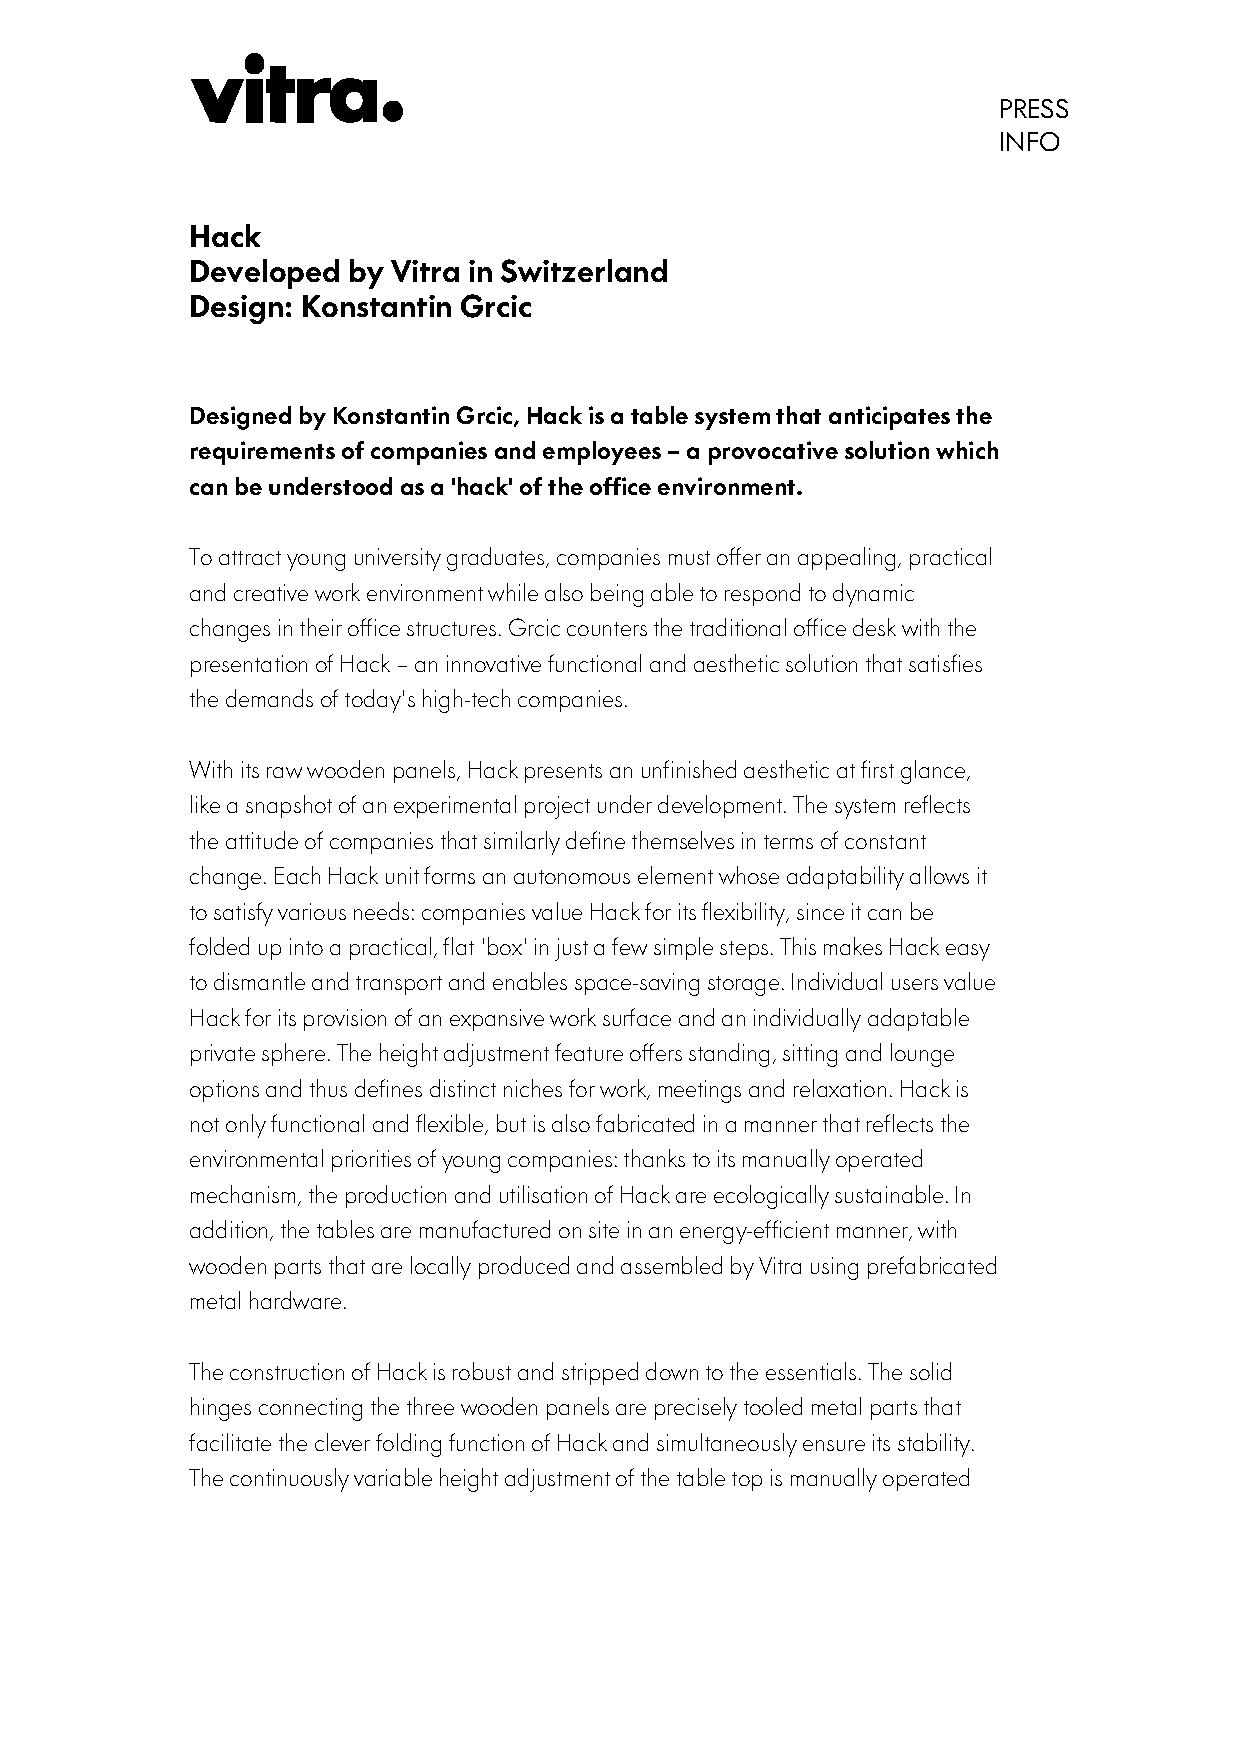
\includepdf[pages={1,2},nup=1x2,scale=0.75]{images/Vitra_Hack}

\begin{figure} \centering

\includegraphics[scale=0.4]{images/Workspirit13HACKStudioAKFB3}

\includegraphics[scale=0.25]{images/HackDeskGrcic} \caption{The Hack Desk,
  designed by Konstantin Grcic, manufactured by Vitra.}
\label{fig:hackdeskimage}
\end{figure}

But the mainstreaming of hackerdom is just as likely to expose the sexism
and/or racism of past communities of hackers.  An ``elite hacker'' in an
interview to an influential hacker zine declared the demise of the hacker
underground with the xenophobic and mysoginistic observation that ``today it
is claimed that the Chinese and even WOMEN are hackers. Man, am I ever glad I
got a chance to experience `the scene' before it degenerated completely''
\parencite{phrackmag_2016}.  Symbolically violent in its own terms, this
observation indexes not only the ethnocentric and gendered lifeworld of most
hacker collectives, but the fact that hacking is no longer limited to the
virtual play-fight among Anglo-American suburban adolescents, pointing also to
questions of personhood with the evaluation of who gets to be considered a
hacker.

What is important to emphasize in these examples is not the adoption of one
definition or another, but the evidence of a series of disparate, conflicting,
and generative differences for the contextualization the hacking. This is the
evidence of an oscillation in respect to the value of ``hacking'' over time:
fluctuating from positive to negative moral valences, that is, from elite,
exclusive groups of technologists to online and offline communities marked by
the rhetoric of opennness and transparency, or, from what the communications'
scholar Douglas Thomas called the ``culture of secrecy'' of the hacker
underground in the height of the Cold War to a ``culture of collaboration,
openness, and transparency'' as a shared utopian horizon in neoliberal times.

\section*{...or hacking?}

What is a hack?  And how is it different from leaks, breaches, exploits, or
other actions of information disclosure and circulation, both constructive and
destructive?

Leaking, for instance, has become associated with hacking in the last decade.
The furor around Wikileaks brought the fun-loving underground anti-collective
Anonymous to world-wide attention via its coordinated attacks on corporations
and governments.  Similarly, piracy: The May 15 movement in Spain was
spearheaded alongside protests of La Ley Sinde---an anti-piracy law widely
opposed by musicians and consumers alike.  These protests ultimately merged with
anti-austerity protests of the ``Indignados'' who shared key activists in the
North African revolutions, who were also involved in the movements organized by
Anonymous, who were often connected to actors in both May15 and Occupy, as well
as hacker activists of many groups including the group ``Telecomix''.  Taken
together, such actions have often been labeled ``hacktivism.''

Hacktivist movements, sometimes autonomous and sometimes part of larger
movements like Occupy, borrow tactics, technologies, slogans and ideas that both
explicitly and implicitly reference the ``hacking'' of Free Software, of the
Pirate Party, of anti-surveillance, pro-privacy hackers (like Tor) and copyright
reform movements like Creative Commons or activists fighting for Net
Neutrality. All of this has occurred at the same time that US and Israeli spies
were infecting Iranian nuclear power plants with the StuxNet virus
\parencite{zetter_countdown_2014}, and the NSA and GHCQ were cataloguing all of
this, and perpetrating some of the greatest ``hacks'' the internet has ever
seen---and this we know mostly because of the even greater intelligence
leak---or ``hack''--- of Edward Snowden.

Hacking, as a practice, is not confined to hackers, but increasingly a practice
essential to the social fabric in surprising ways.  One might turn to ``practice
theory'' in its various forms to explore this---are hackers part of a
``community of practice'' constituted by hacks-as-practice?  Is hacking a
political expression of an emergent sociocultural field, in Bourdieusian terms?
Are hackers heterodox actors in the context of a mainstream computing field,
wildcards in various professional domains, akin to the figure of Luther Blisset
or Guy Fawks who can come in and out of a mysterious identity?  Is hacking now
mainstream itself?

To speak of hackers as a community of practice, or of hacking as a field,
combines questions of technical and political cultivation with the
identification of a distinctive practice in order to suggest that the identity
of a hackers is based in the practice of hacking.  Indeed, such definitions are
common (we ourselves have proposed them---in the case of a ``recursive public''
for instance Kelty \cite*{kelty_two_2008}).  But this approach cannot 
accommodate the fact that hacking and hacks have become more obsteperous 
and unruly in their circulation: hackers fight hackers (vigilante-style or
as collaborators of law enforcement), trolls troll trolls, and pirates steal 
from pirates today.  To conflate the question of hacker identity with the 
question of the practice, political, technical or otherwise, would miss the 
mark.

Instead, there are multiple and intersecting moral and technical orders 
inhabited by people who self-identify or are identified by peers as hackers. 
From the underground hacker collectives to ``grey hat'' security researchers 
to spam-slinging criminal actors, to the hard-core free speech and privacy 
cryptography defenders; from the die-hard Free Software activist to the 
business-oriented Open Source evangelist; from the über-cool Northern 
European design artists to the goofy-but-terrifying Anonymous hackers, 
and so on.  As Coleman and Golub \cite*{coleman_hacker_2008} point out, 
there is no single liberal ideology that hackers adopt, but rather a 
range of ``genres'' in which any given individual or group might 
operate, implying both the freedom and the constraints that word signals.

The notion of genre is useful for integrating hackers and hacks in a complex
whole---a kind of story that integrates elements of personhood with material
forms, technical practices and political rationalities.  But it is also the case
that ``hacks'' can be independent, modified, shared and re-appropriated across
genres.  Hacks imply a range of technological affordances that make practices of
hacking less dependent on embodied skill than many other kinds of practice
(e.g. glass blowing or cabinet making) and as a result more mobile and
modifiable.  The expanded field of hacks, leaks, exploits, breaches, ops, online
campaigns and so on form the very substance of political and working life today
in its complex entanglements with things, protocols, perspectives, and
sensibilities of digital technologists and technologies.

In the next section, therefore, we turn to the question of how one might
distinguish hacks as different forms and expressions of power.  Because hacks
are a regular feature of work, play and politics, it is important to look at the
kinds of hacks that cross these divisions, and represent mutations in the
configuration of power, knowledge and everyday practice in a Foucauldian sense.
Hacking, leaking, breaching, hacktivism, and so on each imply different sets of
tools, tactics and practices, and engage overlapping genres of hackers.
Foucault's approach to power has generally been used to make a claim for certain
general or epochal changes as a result of such mutations in the field of
tactical power: sovereignty, biopower/disciplinary power, and the
governmentality of neoliberalism.  But recent work on Foucault suggests that
reflects his own interest in the mutual confirguation of these different
political rationalities \parencite{Macmillan2011a}.

Instead, we suggest that there are reconfigurable elements in the domains of in
which ``hacking'' is relevant---a ``topology'' in which some forms of
``hacking'' respond to and constrain others.  Hacks are often a recombination of
the elements of power, a stretching of this topology in which action and
response create tensions and thresholds of power related to particular modes of
hacking.  Approached this way, one can better narrate the ``recombination of
elements'' that Foucault (at least later in his work) recognized as a way to
stretch, transform or warp the patterns of correlation that make up a given
mode or configuration of power \parencite{Collier2009a}.

Viewed this way, we can better account for the fact that many ``hacker
practices'' do not originate with hackers, nor do they confine themselves to use
by hackers.  Tactics or practices are picked up by computer security scientists
and researchers, security firms, police forces, political campaigns, anti-piracy
outfits, analysts of all sorts, as well as spreading globally through networks
of activists, hacker and maker spaces, legal firms, musicians and artists, or
consumers and pirates. Hackers go to work for Google or Facebook, anti-piracy
companies appropriate the tools of hackers and pirates.  Pirates hack free
software tools, and large corporations engage in technical and legal
cat-and-mouse games with pirates. Power, in this sense, is about the
recognition, appropriation, recomposition, and redistribution of tactics and
practices: not ideologies or genres as much as recomposable instances of power.  The
technique of DDOS attack, for instance, or the use of a copyright infringement
cease-and-desist letter, the creation of commons-producing copyleft licenses, or
the use of the BitTorrent protocol can all be called hacks, but they look
different when employed in response to other hacks, leaks or breaches.

The first three practices listed here (invention, inversion, and figuration) are
quasi-direct forms of action; they are accessible to anyone and do not require
large investments of money or stable organizations to mobilize.  The last two
(regulatory action and enforcement), however, are often more second-order or
``representative'' in that they often require physical, financial or
organizational resources and a certain scale and depth of involvement to
perform.  But we suggest that even these two forms have a ``hackish'' character
in the contemporary.

\subsection*{Invention}

\textbf{Invention} is the broadest possible meaning of hacking. It includes
building and making things, and not only material things, but especially
so-called ``immaterial'' products such as software, legal licenses, or
organizations.  Invention might include those practices that arise out of a
lack, and at least in the conventional language of research and development, it
comes with extensive planning, study and investment of time and money.  But
considered as a form of ``hacking,'' invention often implies a possibility based
in the existence of multiple existing tools and components.  Creating software,
hacking together hardware components or starting up an organization are all
practices of invention in so far as they are carried out to solve a problem or
respond to a lack that makes certain possibilities clear.

Invention in the era of hacking has become much simpler and cheaper, as
toolkits, frameworks, patterns, and languages and other easily reusable and
either cheap or free to use tools create a material culture of ready-made,
accessible, often lego-like parts.  Easy access to tools is by now an ethic (as
in the case of the Whole Earth Catalog,``Access to Tools'' described by Turner
\cite*{turner_counterculture_2006}) of mutual aid and instruction, and an
appreciation for both the DIY possibilities of our world, and sometimes a
respect for (and desire to contribute to) the coordinated engineering necessary
to bring them into being.

Furthermore, the practice of invention implies an affinity based in shared
understandings of how things work.  Whether that is a classic engineering
culture (based in University and/or corporate practice), a DIY geek culture, a
UNIX culture, a glass-blowing culture \parencite{o2005embodied}, invention
demands not only skill but the capacity to recognized others with more or less
the same skills, habits of practice and commitments to certain kinds of
technological or material choices \parencite{Sennett2008}.  It is this version
of hacking that is most clearly identified with, for instance, the Internet
Engineering communities described above, but also because of its generally
positive valence, the aspect which is emphasized by Silicon Valley start-ups.

\subsection*{Inversion}

\textbf{Inversion} is a term meant to signal a practice that---at least under
the label of ``hacking''---is often insufficiently distinguished from invention.
Inversion is the kind of hacking that involves finding a way to use existing
tools or technologies to achieve something they were not meant to do.  Under
this aspect, exploits of vulnerabilities, using systems against themselves,
inverting the intended purpose of a system, or remixing something for purposes
of critique, parody, ridicule or something more practical
\cite{galloway2007exploit}.  In terms of hardware, it includes the practices of
modding and customization; in terms of software, it includes the practice of
finding and exploiting weaknesses in software (for good or evil intent) or
recombining software elements in a surprising and clever way in order to achieve
a new goal.

A famous example of inversion is neither hardware nor software but a so-called
``legal hack'': the General Public License (GPL), which uses existing statutory
copyright law to accomplish something it was not intended to do.

Inversion generally assumes institutional structures or infrastructures with a
certain transparency (one must be able to see how something works in order to
exploit it).  Some tactics exist for inverting the
non-transparent. Leaking---such as the actions of Wikileaks or Snowden---might
be considered an inversion, as might some forms of reverse engineering of secret
techniques or technologies.  For technologists of the ``hacker underground''
ilk, a whole range of tools exist for attempting to break technologies, either
to gain access, or to control them (the creation of Botnets, zombie servers,
etc.)

Inversion also implies faith in engineering and in the rule of law: for
something to be inverted is not the same as for it to be destroyed or disabled.
GPL licenses work because copyright law is legitimate and enforced.  Remix or
recombination of software is done because the challenge is often to make
something work better or meet higher standards of practice or security.  By
extension, the faith is that things can always be and become better; only
imperfect things can be hacked--- inverted---in this sense.

Similarly inversion implies patterns of regularity that can be exploited---the
very thing upon which the practice of invention often depends as well.
Inversion works upon certain technological or organizational preferences shared
amongst a large group of people---for instance the use of SCADA control systems
amongst process engineers who design large industrial plants allows for hackers
to imagine exploits with powerful effects on the material world.  Similarly,
entrenched social behaviors are often exploited in ``social engineering'' hacks
that rely on the regularities of organizational design and human behavior.

\subsection*{Figuration}

It is also clear to many that not all hacking is restricted to technological
manipulation. We sugest \textbf{figuration} to capture the more traditional and
recognizable forms of political action: rhetorical persuasion, ideological
argument, political advocacy, etc.  Classic descriptions of the functions of the
public sphere tend to characterize it as an issue of sovereignty---the ability
of ``the people'' to speak to and force changes amongst established domains of
power like the state, the church, the military,
etc. \cite{anderson2006imagined}.  All of the tactics involved here are about
visibility and the legitimacy of a political process.

To speak of figuration as a mode or component of ``hacking'' today, however, is
to recognize that such classical forms of discursive and persuasive power are
also used as forms, and in response to, hacking: operations by anonymous, for
instance, can be restricted to the widespread circulation of messages, videos
and manifestos. The protests against SOPA and PIPA in 2012 were largely
traditional responses by hackers (and others) to an attempted regulatory 
action.

Materially speaking, figuration depends on shared communication structures. Very
often today, hacking can take the form of \emph{inventing} or \emph{inverting}
communication practices as part of or in response to practices of figuration.
In many ways, open government data advocates of the last few years are demanding
that longstanding institutional structures (such as public hearings or requests
for comments) be hacked in order to make government similar or more responsive.
To do this they rely on a figuration of government as slow, non-responsive,
elitist or rigidly bureaucratic.

Substantively (at least in the domains of intellectual property and information
technology) practices of figuration have been heavily focused on issues such as
privacy, transparency, free speech, freedom to operate (or innovate) and network
neutrality.  These issues subtend a long and rich discourse that includes both
scholarly debates and conventional understandings of these concepts and their
value to our lives.  Examples of ``hackish'' figuration include the Electronic
Frontier Foundation. EFF was created in the context of ``hacker crackdowns'' of
the early 1990's to articulate a discourse on the importance of defending civil
liberties online, and as a fund to legally defend hackers from prosecutorial
overreach.  Similarly, the death of Aaron Swartz provides a figure of openness
and open access as vital global struggles to which hackers can and should
contribute.

\subsection*{Regulatory action}

\textbf{Regulatory action} is not historically a form of hacking, and in many
ways it is its most important opposite.  Nonetheless, a hackish attitude towards
regulatory action has emerged as a possibility---the strategic attempt to
regulate (either formally as part of government action or through software, or
informally through other means) represents another tool in the hacker kit.  The
language of regulation-as-control was most clearly articulated in terms of
hacking by Lessig's famous work \emph{Code, and other laws of cyberspace}, which
argued that many different kinds of things regulate behavior (law, morals,
architecture) and are amenable to change to different degrees
\cite{lessig2000code}.

At the most general level, regulatory action includes any form of policy change
intended to introduce, maintain or extend control.  State-based forms of
regulatory action are the most obvious and familiar but large corporations also
engage in regulatory action of particular kinds routinely---especially those
industries who control networks or technologies in widespread use.

Regulatory action almost necessarily implies large bureaucratic organizations of
a classic Weberian type---rule-based, hierarchically ordered, and subject to
regimes of oversight and transparency.  As a result, regulatory action is
relatively rare, and comparatively complicated to carry through.  The tactics of
invention, inversion and figuration are often oriented towards influencing,
responding to or disrupting regulatory action of various kinds---the 2012 case
of protests against SOPA/PIPA being a clear case; another case would be
Operation Payback conducted by participants of Anonymous against the global 
credit card companies Mastercard and Visa, who had engaged in the regulatory 
action of systematically blocking PayPal donations to the Wikileaks organization.

% Regulatory action also implies a professional cadre acquainted with the rules
% and procedures of these organizations, oriented towards professional norms of
% democratic governmental practice, even if in practice such norms are honored in
% the breach or routinely subjected to the power of external interests.
% Nonetheless, regulatory action is something that is routinely pursued
% strategically by different groups---a corporation lobbies congress, one groups
% sues another or asks a court for an injunction; lawyers send letters; states
% create new roles and appoint people to them (e.g. IP Czar); courts mete??? out
% punishment, etc.

Inversion often borders on regulatory action when it is used strategically to
achieve something in the interests of a particular entity, but so too does
figuration, which is the tactic most often employed to support or protest
a proposed legal change (both were used in the case of SOPA/PIPA).  Cases of
significant interest include those where regulatory action look more like cases
of inversion---i.e. where a legal action, for instance, is used to threaten,
intimidate or censor a particular group. The injunctions filed against
Megaupload and its owner, Kim Dotcom, for instance, are represented as mere 
enforcement of the law, but in reality represent the effective mobilization 
of state power by industry organizations like the MPAA and the RIAA.

\subsection*{Enforcement(s)}

Finally, there are practices of enforcement. Often only implicitly or
metaphorically included in a Foucauldian analysis (discipline is held to be
more insidious and more profound kind of force, a 'government of the soul' for
instance).  While classic displays of sovereign power are relatively rare
(helicopter raids by anti-terrorist forces on New Zealand mansions of
flamboyant wannabe hackers notwithstanding, such as the case of Kim DotCom), 
they remain a central tactic in the repertoire of power, and they are by no means
restricted to a state and its repressive apparatuses.

Many forms of enforcement are widely available today.  A range of tactics and
practices of which the DDOS is only the most common are not confined to any
particular segment of society, but available to anyone who might, for instance,
download and install a copy of the Low Orbit Ion Cannon (or its predecessor,
FloodNet, written by the Electronic Disturbance Theater group in 1994 to flood
the Mexican government website with requests in order to send a message of
support for the Zapatistas).  Legal tools like cease-and-desist letters are also
routinely used as a tactic of force; even patent litigation can be figured this
way when conducted by so-called patent trolls.  Networked-based forms of
disruption are very often simultaneously tactics of invention or
inversion—coming into existence in response to the actions of states or
corporations.  Piracy and cracking generally might be said to move from being a
tactic of inversion when a vulnerability in a copy-protection scheme is merely
demonstrated (e.g. Sklyarov demonstrating holes in the eBook Reader) to a tactic
of force when that vulnerability is routinely exploited for gain, protest or
sabotage.

\begin{figure} \centering 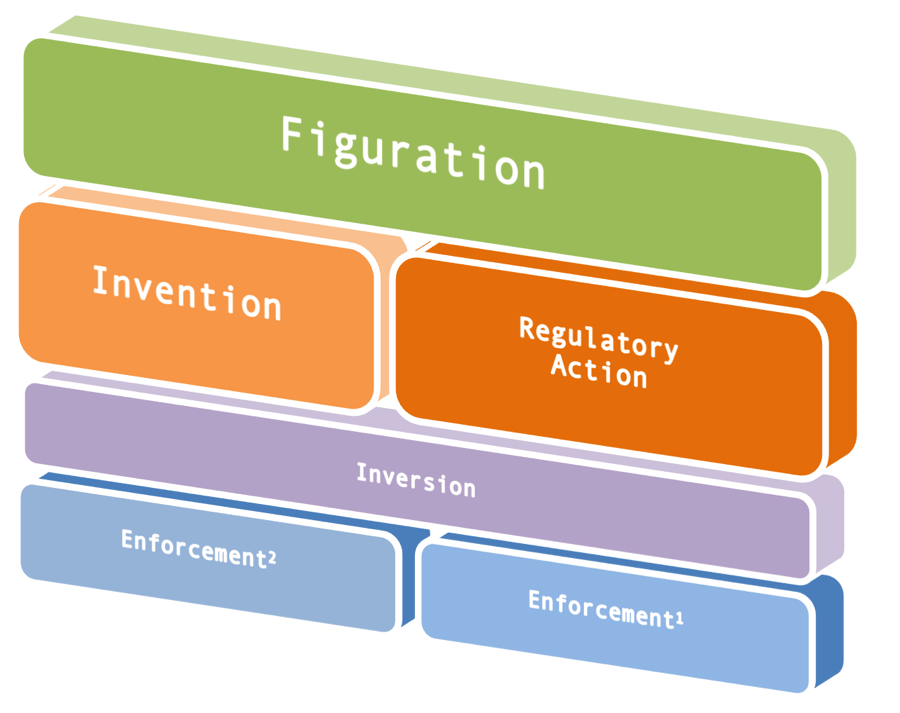
\includegraphics[scale=0.5]{images/protocolstackV2}
\caption{Stack of Power: an analytic decomposition of hacking
practices and how they might relate} \label{fig:ProtocolStack} \end{figure}

These five practices fit together as one possible description of how ``hacking''
is part of a topology of power today.  The software programmer's metaphor
of a ``stack'' is useful here---in common parlance it refers to a frequently
deployed but heterogeneous collection of tools.  Such tools interface with each
other, and can in some cases come to depend on one another (nothing would happen
without an operating system in place, but there are many variants available).

The image of the stack we employ here, however, is meant to provide a basic map
of push and pull, of action and reaction, or of provocation and response.  We
intend it to be used to help diagnose certain technical or political thresholds
in the recent past of hacking (and we take it as axiomatic, as anthropologists, that
hackers are historically situated subjects who experience these thresholds in
their own lives and practices under different conditions, despite sharing many
technical devices, protocols, and infrastructures).   

--> 

%Take for example, the case of Napster, which for many hackers around 2001,
%represented a significant technical and political threshold.  A technical
%threshold because it was an inversion of the normal system of distribution of music.
%It used simple available technologies (the MP3 format, the ability of networked
%computers to share files, and a simple interface) to quickly and more or less
%elegantly demonstrate how the massive, quick and easy sharing of digital musical
%files could be accomplished, almost overnight.  But it was also a political
%threshold because just as quickly, it was shut down by a regulatory action
%initiated by the RIAA---a clear demonstration of the continuing power of law
%over the possibilities of technology.  There followed a war of figuration over
%individuals figured as pirates by the industry, and as music lovers sharing
%music by the proponents of intellectual property reform and technological
%progress.  In response to this threshold, a technology like BitTorrent could
%emerge as something engineered to get around the law---not simply a clever
%invention in its own right, but one that created around certain legal limits. 
%
%Napster was not, however, by any account at the time, a work of hackers.  It was
%not free or open source software, Sean Fanning is often figured more often as
%huckster than as hacker, and it does not figure in most narratives of the
%history of hacking.  And yet the kinds of practices involved---ranging from the
%immediate creation of the software, the use it made of available tools, the
%figuration of the intellectual property wars, and the tide of
%enforcement---take-downs, lawsuits, cease and desist letters and DMCA
%notices---that followed are clearly central to the technical, political and
%moral imaginaries of most hackers.
%
%A similar diagnosis can be made of other cases: the creation of the Electronic
%Frontier Foundation as a response to the CFAA, and the subsequent spread of
%underground ``security'' research as a domain of legitimate hacking.  Or the
%improvement, spread and embrace of Tor in response to the political movements of
%2011 (as well as its use for criminal purposes, as in the case of the Silk Road
%story), and the revelations of NSA spying. 

\section*{Conclusion}

Are we experiencing the distancing between the ``hacker'' as a particular
manifestation of personhood and the ``hack'' as a set of tactics of power? Or,
conversely, are we witnessing a global expansion of the conditions for
cultivation of hacker expertise, leading to a proliferation of differences in
the context of what it means to be a hacker and to hack? How is the global
difference in technical and moral cultivation of computer technologists related
to the global accessibility of hacks?  What are examples of the reverse process
in which the actions of global hackers (say, book pirates in Russia, hacktivists
in Tunisia, or Anonymous' attacks on ISIS) have an impact on mainstream
practices?

To return to these open questions, we conclude with the following observations.
First, we suggest that the study of hacking as a practice of ethical and
technical enskillment can be advanced to describe and interpret manifestations
of hacking outside the Euro-American centers of technical and discursive
production on digital technology.  Such work is necessary if we seek to displace the
imperial imperative of digital technology, which often transforms sociotechnical
\emph{difference} into resemblance (or poorly made copy) in other parts of the
world.

Anthropological studies of the global circulation of digital
technologies and expert technologists have demonstrated the naturalization of
Euro-American assumptions in digital design: from user interfaces to data
models; assumptions of usefulness of particular technologies based on the
prestige of their place of creation; and the imposition of particular projects
from centers of production to disconnected peripheries of the global
South\cite{chan_networking_2013,takhteyev_coding_2012,xiang_2007}.  We suggest
that such assumptions might well be built into the global stack of power we
describe above,  and to look to different traditions would be to ask how hacks
themselves might be hacked.

The recent past of hacking clearly overlaps with other practices--those of 
piracy, activism (whether labeled cyber-activism or hacktivism), trolling, 
leaking and breaching.  Such practices should be understood not simple as 
forms of hacking, but as part of topology of power which is locally stable, 
but historically changing.  If history tends to the stabilization of forms 
of power, the manifest speed and ease with which the contemporary topology 
can be stretched and deformed suggests a perpetual oscillation or turbulence, 
limited only by the energy and enthusiasm that can be committed to the various 
practices of invention, inversion, enforcement or regulation.

Secondly, we suggest that the widespread embrace of hacking reflects changes in
two traditional domains of study: work and political action.  The language of
hacking and the question of hacker personhood provides a window on the changing
meaning of work, career and expertise.  Rather than a life-long career, grounded
in training and acquisition of expertise, maintained through repeated trials of
problem-solving within the basic framework of the division of labor, the embrace
of ``hacking'' (as in the case of the Hack Desk) is clear evidence of anxieties
about features of work that are temporary, flexible, transient, and often highly
individualized ways of demonstrating one's creativity.  They remain focused on
problem-solving, but disdain a division of labor and a hierarchy of expertise,
which often mirrors actual changes in work environments in the last several
decades \parencite{Boltanski2005}.  In this respect, hacker personhood may
represent a vanguard of sorts for changes affecting large parts of a global
labor force.

By contrast, when hacker personhood is considered in light of political action,
it highlights a different set of changes, and possibly a political threshold by
which might be described as a new form of sabotage.  It is this
aspect---especially under the label of hacktivism which raises the central
question of the link between hackers and hacking, precisely because of the
proliferation of hacks that can be simultaneously be used for diametrically
opposed political purposes.  Sabotage does not always imply a form of class
resistance---it is also often a competitive tactic within capitalism and a form
of warfare engaged in by state actors.  But whether this form of
hacking-as-sabotage is related to the production of a particular form of hacker
personhood remains an open question. 

Finally, there are important methodological lessons to be learned by
anthropologists and other social scientists through the study of hacking. The
digital is not a panacea for the problems of collaborative research in
anthropology and the human sciences at large; but it can certainly help if
digital technologies are redesigned to further promote collaborative engagements
between ourselves and with the communities with we conduct research. Digitization
of field research carries potential benefits with respect to the ease of
archival and data sharing, allowing for longitudinal and extensive comparative
studies.  But it also carries serious issues of data privacy and anonymity as
most researchers (in both the sciences and humanities) are not well informed and
trained to handle problems of information security.  Hacking, in this regard, is
an important source of practices and workarounds, both in the sense of invention
and inversion, to deal with questions of information security, but also sharing
and remote collaboration across transnational lines of exchange.


\section*{Further References}

\begin{itemize}
\item  Original MIT Jargon File, kept by Paul Dourish:
  http://www.dourish.com/goodies/jargon.html 
\item  Extended Jargon File at Eric Raymond's site:
  http://www.catb.org/jargon/html/
\item Jason Scott's textfiles:
  http://textfiles.com/ 
\item Hackerspaces wiki: 
  http://hackerspaces.org
\end{itemize}

%\bibliography{hack_entry} \bibliographystyle{agsm}

\printbibliography 


\end{document}

